\section{Results}
\label{sec:results}

In the following, the molar heat capacity and then the Debye temperature are determined

\subsection{Parameters}
\label{sec:parameters}

The copper sample in this experiment has a mass of $m = \qty{0.342}{\kilo\gram}$ \textnormal{\cite{molar_heat}} and a density of
$ \rho = \qty{8930}{\kilo\gram \per \meter^3 }$ \textnormal{\cite{kupfer}}.
The table \ref{tab:parameters} shows the molar volume and the compression modul of copper.
%erstelle tabelle
\begin{table}[H]
	\centering
	\caption{Parameters of the copper sample}
	\label{tab:parameters}
	\begin{tabular}{c c }
		\toprule
		Parameter & Value \\
		\midrule
		$V_m$ & $\qty{7.11e-6}{\meter^3 \per \mol}$ \cite{chemie_kupfer}\\
		$\kappa$ & $\qty{140} {\giga\pascal}$ \cite{perioden_kupfer}\\
		\bottomrule
	\end{tabular}
\end{table}

The molar mass, the number of moles and the number of particles can then be calculated.
The following applies to the molar mass
\begin{equation*}
	M = V_m \cdot \rho = \qty{0.0634}{\kilo\gram \per \mol}.
\end{equation*}

The number of moles is calculated as follows
\begin{equation*}
	n = \frac{m}{M} = \num{5.103}
\end{equation*}

The result for the number of particles is
\begin{equation*}
	N = n \cdot N_A = \num{3.07e24}.
\end{equation*}

The transverse velocity of sound and the longitudinal velocity of sound are also required for further calculations.
These are $v_t = \qty{2260}{\meter \per \second}$ and $v_l = \qty{4700}{\meter \per \second}$ \cite{molar_heat}.

\subsection{Theoretical Debye Temperature}
\label{sec:theoretical_debye_temperature}

The Debye temperature is calculated using the formula %\ref{eq:debye_temperature}.

\begin{figure}[H]
	\centering
	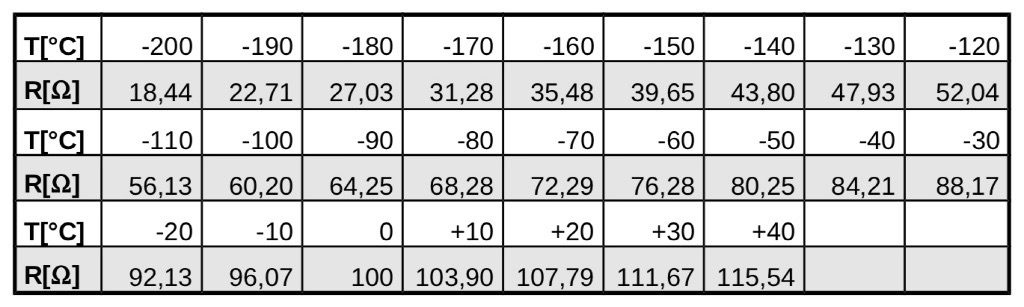
\includegraphics[width=0.6\linewidth]{content/graphics/resistance.jpg}
	\caption{\cite{molar_heat}}
	\label{fig:resistance}
\end{figure}

\begin{figure}[H]
	\centering
	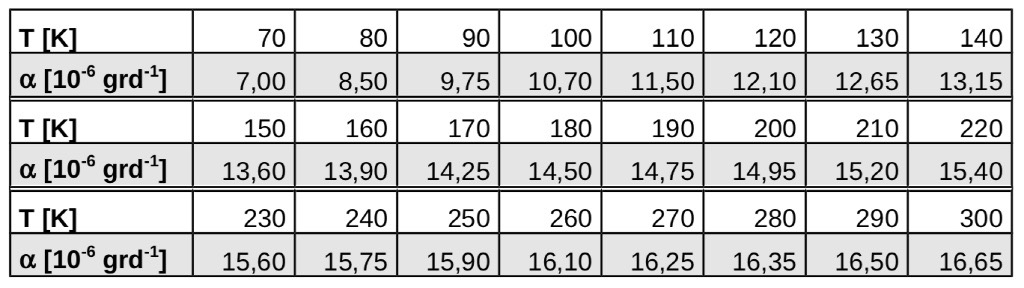
\includegraphics[width=0.6\linewidth]{content/graphics/expansion.jpg}
	\caption{\cite{molar_heat}}
	\label{fig:expansion}
\end{figure}

\begin{figure}[H]
	\centering
	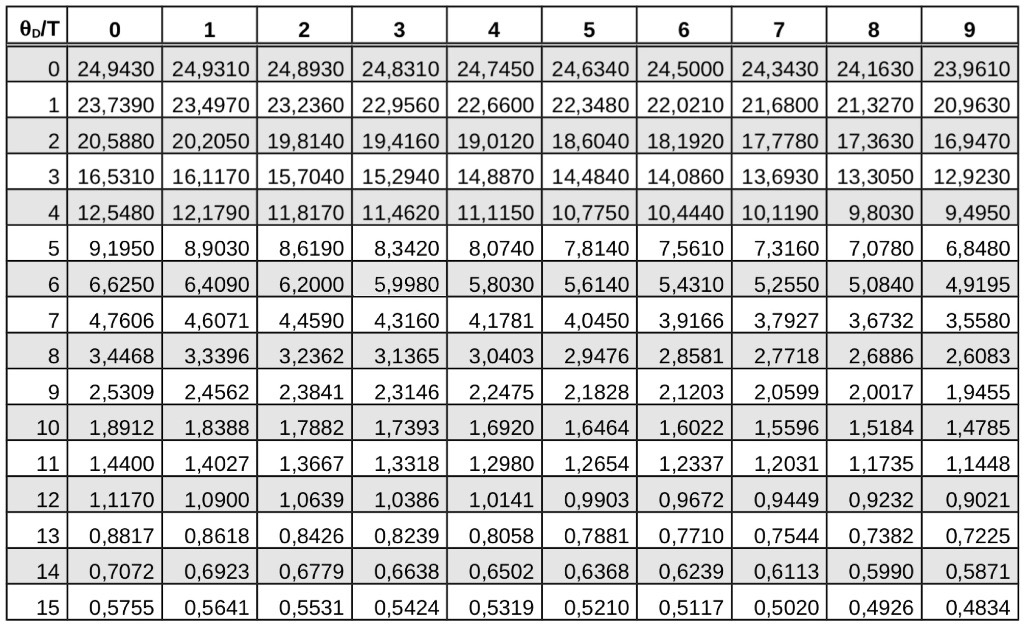
\includegraphics[width=0.8\linewidth]{content/graphics/ratio.jpg}
	\caption{\cite{molar_heat}}
	\label{fig:ratio}
\end{figure}
